\documentclass{pgnotes}

\title{Cooling}

\begin{document}

\maketitle

Recommended background reading from the APC white paper library \href{https://whitepapers.apc.com/}{APC white papers}:
%\begin{itemize}
%\item APC white paper 57 \citep{evans:2014:fundamental}
%\item APC white paper 59 \citep{evans:2012:the-different}
%\item APC white paper 68 \citep{rasmussen:2020:cooling}
%\end{itemize}

Heat removal is necessary for all data centre environments, from tiny closets to large multi-acre dedicated facilities.
Almost all the electrical power input to IT equipment is converted to heat.
Without any means to remove heat, the temperature in the closed space will rise quickly.

\section{Temperature}

Temperature quantifies how hot an environment is.

In Europe, temperature is usually expressed in Celsius (formerly Centigrade) unit.
The Fahrenheit scale (\si{\fahrenheit}) is sometimes encountered in US-centric publications about cooling systems.

\begin{table}[htbp]
  \centering
  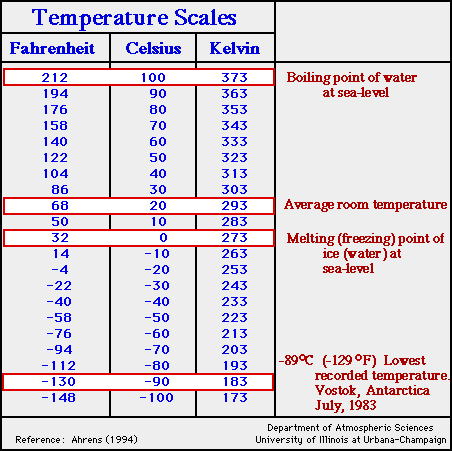
\includegraphics[width=1.0\linewidth]{temp_scales_ahrens}
  \caption{Temperature Scales (Ahrens 1994)}
  \label{tab:temp-scales}
\end{table}

\subsection{Temperature conversions}

The most common conversion is to/from Fahrenheit.
\begin{align}
  T_C & = \frac{T_F-32}{1.8} \label{eq:f-to-c} \\
  \Rightarrow  T_F & = T_C \times 1.8 + 32 \label{eq:c-to-f}
\end{align}

The Kelvin scale is rarely encountered in applied cooling work but is directly related to the Celsius scale:
\begin{align}
  T_C & = T_K - 273 \label{eq:k-to-c} \\
  T_K & = T_C + 273 \label{eq:c-to-k} 
\end{align}

\section{Thermal envelope}

Equipment and humans can only tolerate a certain range of temperatures, or thermal envelope.
If IT equipment is operated outside of its thermal envelope it can lead to CPU throttling, thermal shutdown and reduced long-term lifespan.

The American Society of Heating, Refrigeration and Air conditioning Engineers (ASHRAE) have published a number of standards for thermal envelopes of data centre environments.
The most recent guidelines published in 2011 are given in \autoref{tab:ashrae-2011-guidelines}.
\begin{table}[htbp]
  \centering
  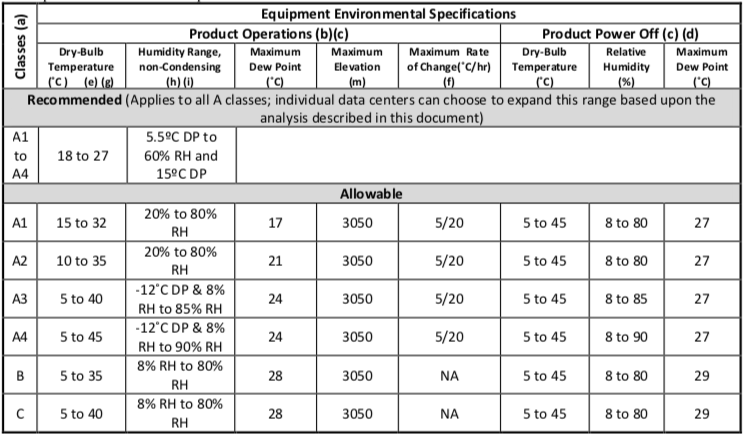
\includegraphics[width=1.0\linewidth]{ashrae_2011_guidelines_celsius}
  \caption{ASHRAE 2011 Guidelines}
  \label{tab:ashrae-2011-guidelines}
\end{table}
Classes A1 to A4 represent normal data centre environments, where environmental controls (e.g. cooling) are used.
The ASHRAE recommended thermal envelope is between 18 and 27 degrees.

\section{Cooling methods}

In order to keep the temperature and relative humidity within permitted limits, we must rely on some method of cooling.

\begin{description}
\item[Conduction] uses the room's surfaces to remove heat to the surrounding building.
\item[Passive ventilation] involves vents placed appropriately within the room to permit hot air to flow naturally out, to be replaced by cooler incoming air.
\item[Fan-assist ventilation] works similarly to passive ventilation, but the air movement is assisted by a fan.
\item[Dedicated cooling] is where the room air is not ventilated, but instead heat is removed from it. 
\end{description}

\subsection{Cooling method selection}

\autoref{fig:cooling-methods} shows the available cooling methods for smaller data centres and server rooms.
As the IT Load increases in size, we often require dedicated cooling solutions.

\autoimage*{cooling_method_guide}{Cooling methods (APC)}{cooling-methods}

\subsection{Fan-assisted ventilation}

Fans can be used on in smaller data centre environments to keep the temperature under control by exchanging the air with the ambient / outside environment, \autoref{fig:fan-assisted-ventilation}.

\autoimage{fan_assisted_ventilation}{Fan-assisted ventilation}{fan-assisted-ventilation}

Fans can be thermostatically controlled.
They can be powered from a UPS to ensure the fans run even when mains power fails. 

In practical terms, anything more than a simple closet with a few devices will need refrigerated cooling.
Conduction, passive ventilation and fan-assisted cooling schemes are ultimately limited by the outdoor temperature.
Consider trying to keep a room at 22C when the outdoor temperature is 34C!


\section{Refrigeration cycle}

The only way to make heat ``flow uphill'' from cold to hot is to assist it.
From our point of view, we want to remove heat from our computer room and reject it to the atmosphere, to keep the room temperature under control.
\autoref{fig:refrigeration-cycle} shows the basic refrigeration cycle.
For a more thorough treatment, see \citet{evans:2014:fundamental}.

\autoimage{refrigeration_cycle}{Refrigeration cycle}{refrigeration-cycle}

There are \textbf{four stages} evident in \autoref{fig:refrigeration-cycle}:
\begin{enumerate}
\item Cold liquid refrigerant in the \textbf{evaporator} is warmed by air passing over it, and boils at roughly \SI{7.8}{\degreeCelsius}. The air passing over the evaporator gives up some of its heat energy. It leaves at a cooler temperature than it entered at.
\item The \textbf{compressor} increases the pressure of the gaseous refrigerant, greatly increasing its temperature to over \SI{50}{\degreeCelsius}.  In doing so, it also acts as a pump for the refrigerant around the loop, which is carrying the heat energy to reject.
\item Hot gaseous refrigerant enters the \textbf{condenser} coil, across which is circulated outside air. As the refrigerant is hotter than the outside air, it gives up its heat to the outside air.  The air passing over the condenser receives heat energy from the hot refrigerant, leaving at a warmer temperature than it entered at. The refrigerant is cooled below its boiling point and changes phase to a liquid.  It will still be quite hot to the touch!
\item The warm liquid flows through the \textbf{expansion valve}, which limits the flow of refrigerant such that it is boiled off in the evaporator. When the refrigerant emerges from the expansion valve, it expands since the flow is limited, and is ready for another cycle in the evaporator. 
\end{enumerate}

Watch the \href{https://www.youtube.com/watch?v=VJX0LyxRV0E}{Refrigeration Cycle 101 video on YouTube}

\newpage

\section{Types of cooling}

\begin{description}
\item[Comfort cooling] is what we are familiar with as air conditioning. Warm humid air in an occupied space is cooled and dehumidified. Usage varies with season and personal preferences.
\item[Precision cooling] is designed to work 24/7 365 days a year to keep temperature (and often humidity) within a set band for IT equipment to work effectively. 
\end{description}

There are two main categories of cooling system seen in data centre environments, direct expansion (DX) and chilled water.

\newpage

\section{Computer Room Air Conditioners}

Refrigerated cooling is provided in a data centre environments by two main families of equipment: Direct eXpansion (DX) and Chilled Water.
DX systems where the evaporator directly meets air in the data centre environment are the simplest to understand and most common in small and medium environments.

DX systems normally take the form of a \textbf{Computer Room Air Conditioner}, or CRAC.
A CRAC is normally a large floor-standing unit containing the evaporator coil, blower fan, compressor and other components.
For in-depth information refer to \citet{evans:2012:the-different}.

\autoimage{crac_photo}{Photo of a Computer Room Air Conditioner}{crac-photo}

CRACs are most usually seen in so-called downflow configuration as in \autoref{fig:cooling-airflow}.
\autoimage{cooling_airflow}{Airflow from Downflow CRAC through raised floor}{cooling-airflow}
\begin{itemize}
\item Warm \textbf{return air} enters the CRAC via an opening on the top of the unit.
  Sometimes the return air is ducted to the unit from above the ceiling.
\item Cold \textbf{supply air} leaves the CRAC via an opening in the bottom:
  \begin{itemize}
  \item If there is a raised floor, the cold air is blown out the bottom of the unit under the raised floor.
    It flows under the raised floor and exits through perforated tiles.
  \item In the case of a solid floor, the cold air normally leaves via a large grille on the bottom of the unit.
  \end{itemize}
\end{itemize}
Other configurations include upflow (reverse of the above, but only on a solid floor), horizontal and other configurations.
Cooling units are sometimes located in other areas and ducted to the data centre environment.

For the cooling system to work properly, we \textbf{must use a hot aisle / cold aisle arrangement}.
Where a raised floor is used, the perforated tiles must be in the cold aisle, and not in the hot aisle.

CRAC evaporator fans normally run continuously.
The refrigeration system cycles on and off under thermostatic control to maintain the selected temperature.
Control is often based on the return, supply or space air temperature.
More sophisticated control strategies are becoming common, but the basic idea outlined above is sufficient.

\newpage

\subsection{Self-contained air-cooled DX}

Self-contained units have all refrigeration components within the CRAC's casing.
The condenser supply and exhaust are ducted from the outdoors.
Limited in cooling capacity to approx \SI{15}{\kilo\watt} due to unit size and ducting, \autoref{fig:crac-dx-self-contained}.

\begin{figure*}[hptb]
  \centering
  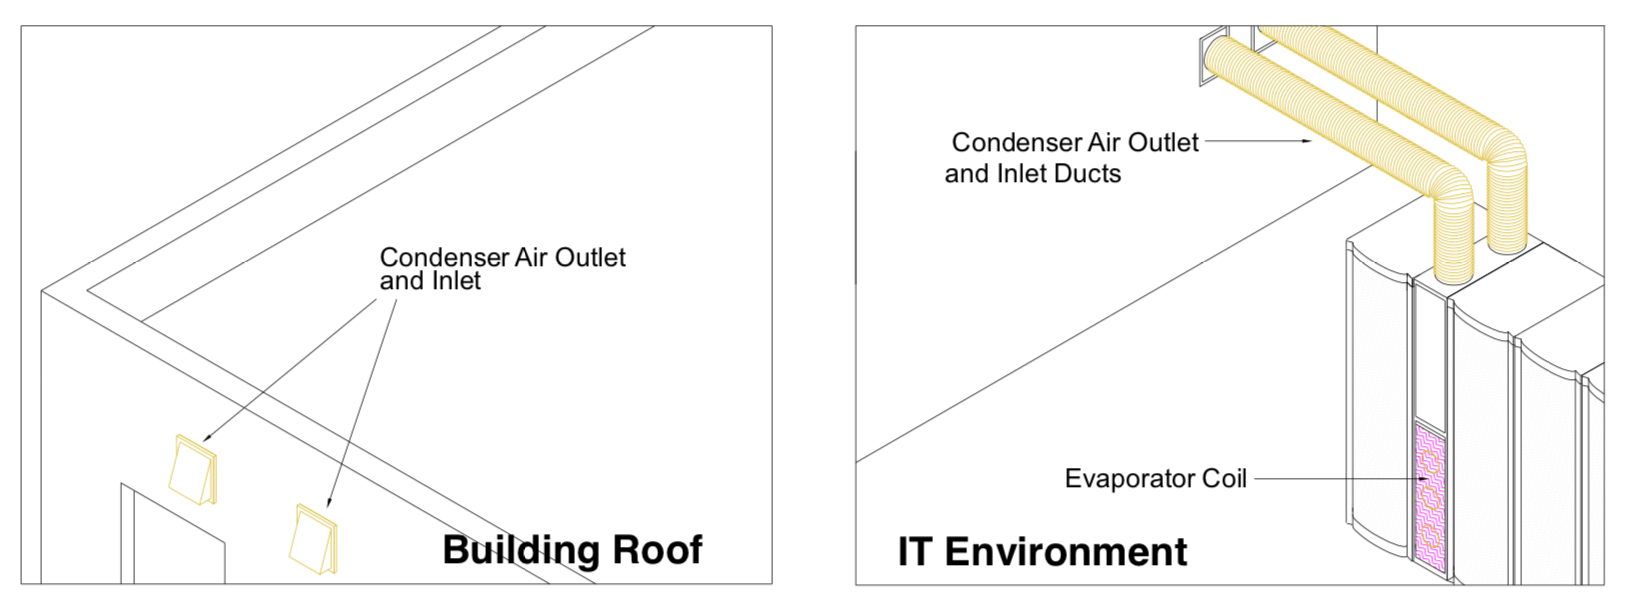
\includegraphics[width=1.0\linewidth]{crac_self_contained_schematic}
  \caption{DX self-contained CRAC (APC)}
  \label{fig:crac-dx-self-contained}
\end{figure*}

Candidate for up to \SI{15}{\kilo\watt}.
Often seen in small on-site server rooms.

\subsection{Air-Cooled DX}

Direct expansion, often abbreviated DX, cooling systems house the evaporator, compressor and expansion valve within the CRAC unit.
The condenser is sited externally, with wiring and refrigerant connections from the CRAC unit, \autoref{fig:crac-dx-air}.

\begin{figure*}[hptb]
  \centering
  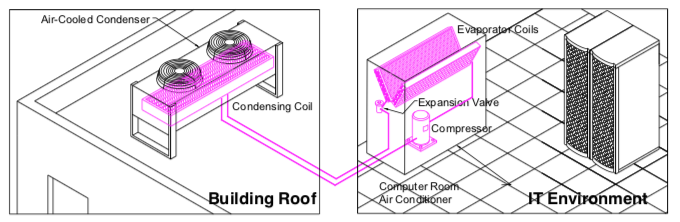
\includegraphics[width=1.0\linewidth]{crac_dx_air_schematic}
  \caption{DX air-cooled CRAC with condenser (APC)}
  \label{fig:crac-dx-air}
\end{figure*}

Candidate for \SIrange{7}{200}{\kilo\watt}.
Multiple units often used for larger capacities and to provide redundancy (see later).

\autoimage{condenser_photo}{Condenser}{condenser-photo}

An alternative layout of the Air-Cooled DX system has the compressor is located in the outdoor unit, called a \textit{condensing unit}.
This arrangement is commonly called the \textit{split system}.

\newpage
\subsection{Glycol-cooled DX}

The Glycol-cooled DX replaces the air-cooled condenser with a refrigerant-to-fluid condenser inside the CRAC casing, \autoref{fig:crac-dx-glycol-dry-cooler}.
Liquid coolant consisting of water mixed with ethylene glycol is circulated between the condenser and a \textit{dry cooler} (coil with a fan) by a \textit{pump package}.

\begin{figure*}[hptb]
  \centering
  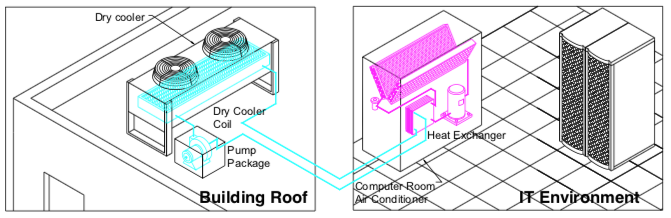
\includegraphics[width=1.0\linewidth]{crac_dx_glycol_schematic}
  \caption{DX Glycol-cooled CRAC with Dry Cooler (APC)}
  \label{fig:crac-dx-glycol-dry-cooler}
\end{figure*}

\autoimage{dry_cooler_photo}{Dry cooler photo}{dry-cooler-photo}

Some advantages of this system are:
\begin{itemize}
\item Refrigeration circuit is sealed inside the CRAC.
\item Glycol can be pumped much longer distances.
\item Can bypass the refrigeration system if the ambient air is cool enough. Glycol pumped through an economizer coil instead. See later on!
\end{itemize}

Candidate for \SIrange{30}{1000}{\kilo\watt}, and where distance exceeds ?? metres.
Systems can either be:
\begin{description}
\item[Unitary] where a single CRAC is linked to a single dry cooler.
\item[Shared] where a number of CRACs share one or more dry coolers.
\end{description}

\newpage
\subsection{Water-cooled DX}

The Water-cooled DX is similar to the glycol-cooled version, except that a water loop is used instead of a glycol loop.
The dry cooler is replaced with a \textit{cooling tower}, often on the facility's roof, where jets of water are cooled by spraying them into a moving air stream. 

\begin{figure*}[hptb]
  \centering
  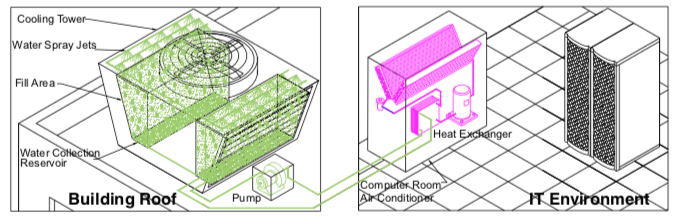
\includegraphics[width=1.0\linewidth]{crac_dx_water_schematic}
  \caption{DX water-cooled CRAC with cooling tower (APC)}
  \label{fig:crac-dx-water-schematic}
\end{figure*}

It is more efficient that Glycol-based systems in hot dry climates, where evaporation in the cooling tower assists with its operation.
However, the water treatment must be carefully considered.
There is also a strong risk of legionella in these systems if not properly looked after.

Water cooled DX is rarely installed in a unitary fashion.
One or more shared cooling towers servicing multiple CRACs with cooled water is by far the most common configuration.

Cooling towers are often operated by facilities management or by the landlord in larger buildings, and water is supplied metered or unmetered ``as a service''.
The same towers often serve not only technical cooling, but also comfort cooling, process cooling and refrigerated storage (for food and other products) systems.


\newpage
\section{Chilled Water Cooling Systems}

Chilled water cooling systems involve the supply of chilled water to Computer Room Air Handlers (CRAH) in the data centre environment.
CRAHs are similar to CRACs in appearance, and are available in the same wide range of airflow configurations.
They are simpler than CRACs, containing only a blower fan, finned water coil and controls.

\autoimage{crah_side_view}{CRAH side view}{crah-side-view}

The chilled water is produced in a separate \textit{chiller}.
The chiller rejects heat from the chilled water loop to the atmosphere in similar ways to DX CRACs.
Air-cooled, glycol-cooled and water cooled chillers are all very common.

\begin{figure}[htbp]
  \centering
  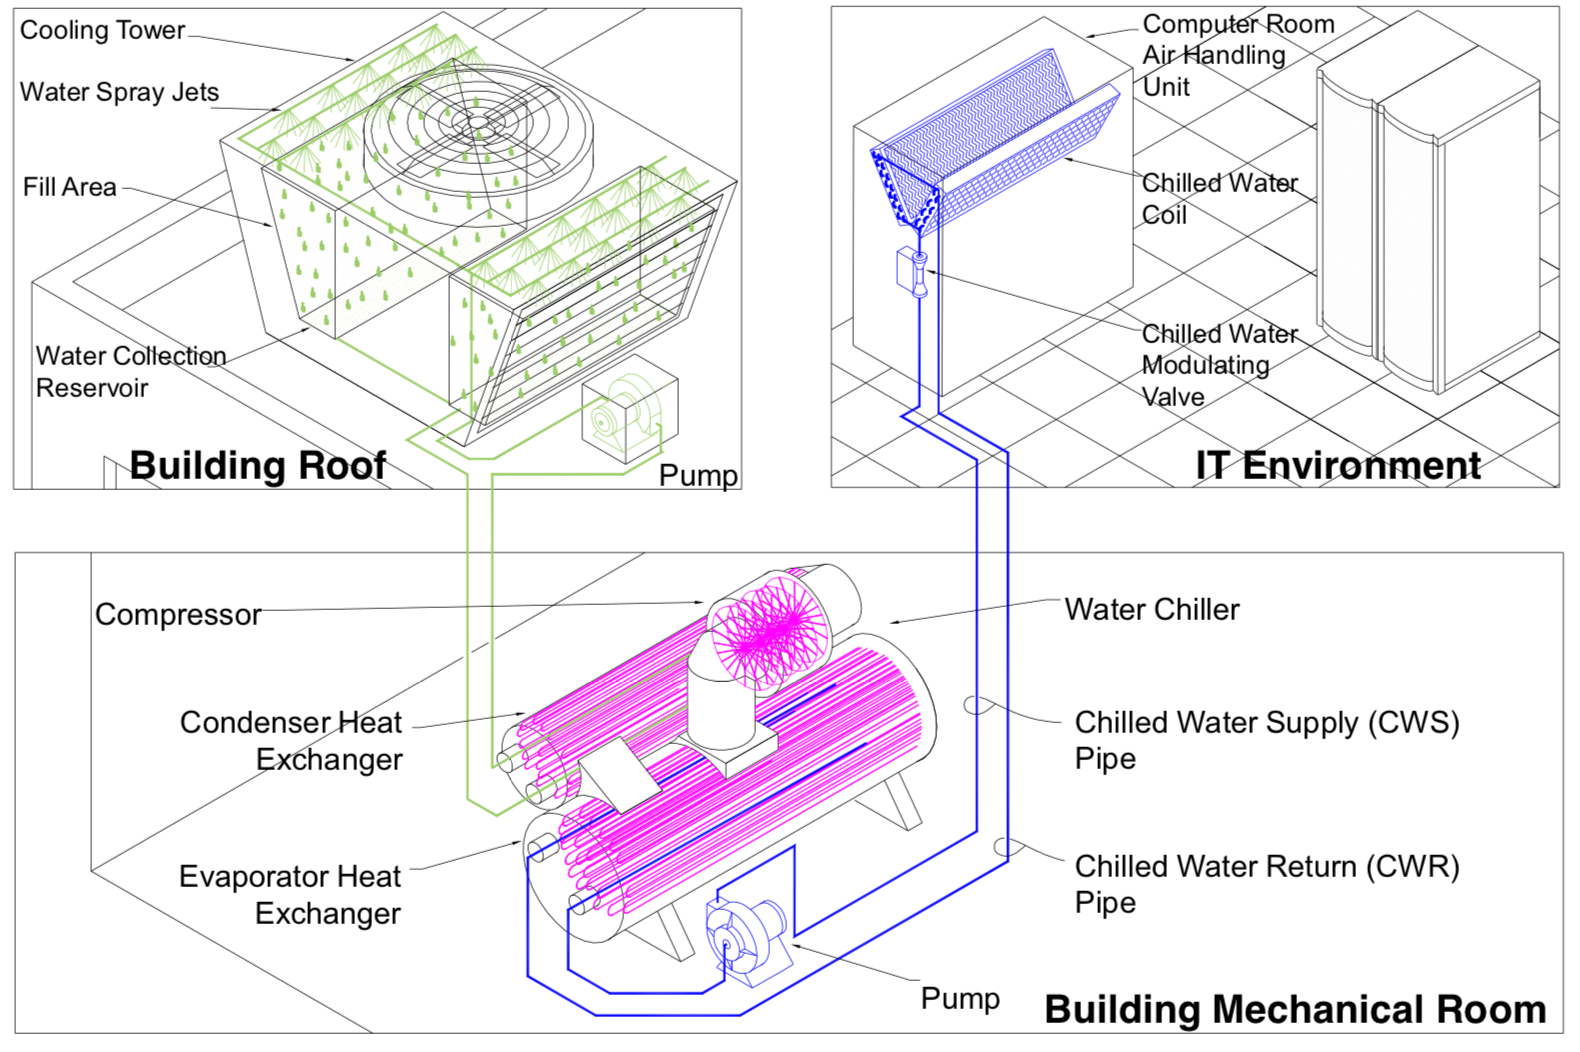
\includegraphics[width=1.0\linewidth]{chilled_water_system_water_cooled}
  \caption{Chilled water system}
  \label{fig:chilled-water-system-water-cooled}
\end{figure}

Although \autoref{fig:chilled-water-system-water-cooled} depicts a unitary system, chilled water systems are almost always installed such that a large number of CRACs or other cooling loads are served by a small number of chillers and cooling towers / fluid coolers.
Chilled water systems also can incorporate large buffer tanks for load balancing, energy price optimisation and to provide \textit{ride through} in case of power failure.

Many buildings, particularly city skyscrapers, use centralised water-cooled chilled water system. 
A small number of very large cooling towers serve a number of chillers which supply chilled water for data centre, comfort cooling and other cooling purposes.
These are generally managed by facilities personnel. 

In a multi-tenant building, the landlord will often supply chilled water as a metered chargeable service to tenants.
Condenser loop water is often also available at a much cheaper unit rate (which can be used for a DX water-cooled CRAC or local water-cooled chiller for IT purposes).

\section{Sizing}

Generally, we total up the IT loads and pad the result by 30\%.

\newpage
\section{Efficiency metrics}

\subsection{Coefficient of Performance (COP)}

The coefficient of performance indicates how many \si{\kilo\watt} of heat is removed per \si{\kilo\watt} of electrical power input to the air conditioning system.
It is calculated as:
\begin{align}
  \mbox{COP} & = \frac{\mbox{cooling power in kW}}{\mbox{cooling system electrical input in kW}}
\end{align}
The COP has no units since the numerator and denominator have the same units.


\subsection{British Thermal Units}

Heat is a form of energy, the SI unit of which is the Joule, \si{\joule}.
When a given amount of energy is transferred per second (e.g. \SI{1}{\joule\per\second}), it is given the unit of the Watt, \si{\watt}.

Many ideas around refrigeration and air conditioning originated from the United States, where imperial units are still common.
In the imperial system, energy is measured in the British Thermal Unit, or BTU.
Power is measured in \si{\BTU\per\hour}. 

To convert from \si{\kilo\watt} to \si{\BTU\per\hour}, we use the relation:
\begin{align}
  \SI{1}{\kilo\watt} & = \SI{3412.142}{\BTU\per\hour}
\end{align}

\subsection{Energy Efficiency Ratio (EER)}

The EER is normally calculated as:
\begin{align}
  \mbox{EER} & = \frac{\mbox{cooling power in btu/hr}}{\mbox{cooling system electrical input in W}}
\end{align}
The EER has units of \si{\BTU\per\hour\per\watt}, but the unit is often omitted.


Note that the EER and COP are directly related by the factor:
\begin{align}
  \EER & = 3.412 \times \COP
\end{align}

\subsection{Power Usage Effectiveness}

The power usage effectiveness (\PUE) of a data centre environment is:
\begin{align}
  \PUE & = \frac{\mbox{total power input to the data centre}}{\mbox{total power input to IT equipment}} \\
       & = 1 + \frac{\mbox{non-IT power input}}{\mbox{IT power input}}
\end{align}
The \PUE is a dimensionless number.
An ideal \PUE would be 1.

\end{document}




